% ======================================================================
%  Four-page IEEE conference paper (IEEEtran). Single file for Overleaf.
%  Upload fig_backrest.png and fig_harmony.png next to this file to show
%  the two result figures; without them a boxed placeholder is printed.
%  Compile with pdfLaTeX. Replace the author/affiliation placeholders.
% ======================================================================
\documentclass[conference]{IEEEtran}
\IEEEoverridecommandlockouts

\usepackage{cite}
\usepackage{amsmath,amssymb}
\usepackage{graphicx}
\usepackage{booktabs}
\usepackage{array}
\usepackage{url}
\usepackage{textcomp}
\usepackage{tikz}
\usetikzlibrary{arrows.meta,positioning,calc}

\def\BibTeX{{\rm B\kern-.05em{\sc i\kern-.025em b}\kern-.08em
    T\kern-.1667em\lower.7ex\hbox{E}\kern-.125emX}}

% optional figure: print the image if the file exists, else a placeholder box
\newcommand{\optfig}[2]{%
  \IfFileExists{#1}{\includegraphics[width=\columnwidth]{#1}}%
  {\fbox{\parbox[c][#2][c]{0.9\columnwidth}{\centering\footnotesize [image \texttt{#1} not uploaded]}}}}

\begin{document}

\title{Text-Driven Room Composition from Catalogue Photos:\\
A Digital Image Processing Pipeline with Guided 2D/3D Chair Recline and Spacing Control}

\author{\IEEEauthorblockN{Aditya Arya}
\IEEEauthorblockA{\textit{Department of [Department]} \\
\textit{[Institution]}\\
[City, Country]}
\and
\IEEEauthorblockN{[Teammate Name]}
\IEEEauthorblockA{\textit{Department of [Department]} \\
\textit{[Institution]}\\
[City, Country]}
}

\maketitle

\begin{abstract}
We present a small, explainable Digital Image Processing (DIP) system that turns a short text prompt such as ``cozy reading corner'' into a composed room image built from real catalogue photographs, and into a rotatable 3D room. Product photos from the Amazon Berkeley Objects (ABO) dataset are enhanced with classical operations (resampling, median and Gaussian filtering, gray-world white balance, CLAHE), cut out with Otsu thresholding, morphology and GrabCut, and compared against a pre-trained U2-Net used as a reference mask. CLIP embeddings retrieve candidates, k-means palettes in CIELAB feed a hue-and-chroma harmony score, and the composition uses placement rules, Reinhard colour transfer, Gaussian shadows and alpha blending. Two interactive geometric edits act on the generated image without calling any model: horizontal object spacing defined on opaque bounding boxes, and a guided backrest-only recline implemented as a piecewise-affine warp on premultiplied alpha that also drives a proxy 3D chair. On 1\,485 products, CLIP reaches NDCG@10 of 0.856 against 0.341--0.696 for colour, shape and texture descriptors; gaps are reproduced to the pixel for all 56 object-class pairs; and an edit takes about 18\,ms once layers are cached. We also report two limits: harmony mostly selects neutral products, and the recline is a 2D projection, not recovered geometry.
\end{abstract}

\begin{IEEEkeywords}
digital image processing, image retrieval, colour harmony, affine transformation, alpha compositing, image segmentation, CLIP
\end{IEEEkeywords}

\section{Introduction}
Online shops show one product at a time on a white background, so a shopper cannot see how a sofa, a lamp and a rug look together. We build a system that composes catalogue photos into a room from a short text prompt, and lets the user adjust the result with simple, explainable image operations. The project was designed around a Digital Image Processing course: every stage uses a standard operation from the syllabus (enhancement, filtering, colour spaces, thresholding, morphology, clustering, geometric transformation, alpha compositing), and pre-trained deep models are used only for text--image matching and as a segmentation reference.

Our contributions are: (i) a complete, CPU-friendly pipeline from catalogue photos to a 2D room image and a 3D proxy room, with per-stage measurements; (ii) a colour-harmony score from CIELAB palettes and an honest analysis of what it optimises; (iii) two geometric edits of the generated image, a measured edge-to-edge spacing control and a guided backrest recline, both specified as explicit affine matrices; and (iv) a verification procedure that measures the edits from rendered pixels. The 3D room is built from simple proxy shapes coloured from the chosen products; it is not a reconstruction of the photographed items.

\section{Related Work}
\textbf{Data and retrieval.} ABO provides catalogue images, metadata and 3D models for household products~\cite{abo}. CLIP embeds images and text in one space~\cite{clip}; we use its OpenCLIP implementation~\cite{openclip}. Classical descriptors for colour, shape and texture include HSV histograms, HOG~\cite{hog} and LBP~\cite{lbp}; we use them as baselines. Ranking quality is measured with NDCG~\cite{ndcg}.

\textbf{Segmentation and enhancement.} We use Otsu's threshold~\cite{otsu}, morphology and GrabCut~\cite{grabcut}; U2-Net~\cite{u2net} serves as a pseudo ground truth. CLAHE~\cite{clahe} and gray-world balance enhance the photos. Textbook coverage follows Gonzalez and Woods~\cite{gw}.

\textbf{Colour and layout.} Colour harmonisation by hue templates was formalised by Cohen-Or \emph{et al.}~\cite{harmonization}; Reinhard \emph{et al.} transfer colour by matching channel statistics~\cite{reinhard}. Furniture layout from design guidelines was studied by Merrell \emph{et al.}~\cite{merrell}. Alpha compositing follows Porter and Duff~\cite{porterduff}; piecewise-affine mappings are classical in image registration~\cite{goshtasby}.

\section{Method}
Fig.~\ref{fig:pipeline} shows the pipeline. Heavy work runs once offline and is stored as 1\,485 RGBA cut-outs, descriptors and palettes (about 30\,MB); the app then needs only these files and the CLIP text encoder.

\begin{figure}[t]
\centering
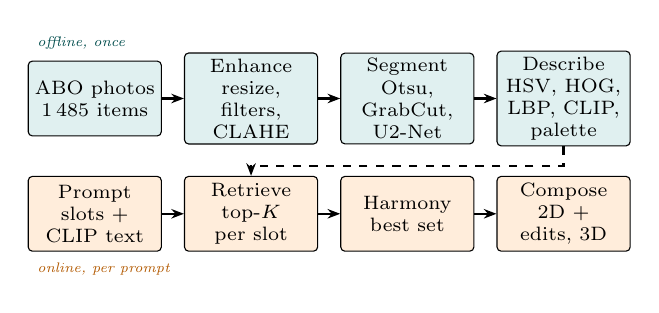
\begin{tikzpicture}[
  font=\scriptsize,
  box/.style={draw, rounded corners=1.5pt, align=center, text width=1.55cm, minimum height=0.95cm, inner sep=2pt, fill=gray!8},
  off/.style={box, fill=teal!12},
  on/.style={box, fill=orange!14},
  arr/.style={-{Stealth[length=1.6mm]}, thick}]
\node[off] (a) {ABO photos\\1\,485 items};
\node[off, right=0.28cm of a] (b) {Enhance\\resize, filters, CLAHE};
\node[off, right=0.28cm of b] (c) {Segment\\Otsu, GrabCut, U2-Net};
\node[off, right=0.28cm of c] (d) {Describe\\HSV, HOG, LBP, CLIP, palette};
\node[on, below=0.5cm of a] (e) {Prompt\\slots + CLIP text};
\node[on, right=0.28cm of e] (f) {Retrieve\\top-$K$ per slot};
\node[on, right=0.28cm of f] (g) {Harmony\\best set};
\node[on, right=0.28cm of g] (h) {Compose\\2D + edits, 3D};
\draw[arr] (a)--(b); \draw[arr] (b)--(c); \draw[arr] (c)--(d);
\draw[arr] (e)--(f); \draw[arr] (f)--(g); \draw[arr] (g)--(h);
\draw[arr, dashed] (d.south) -- ++(0,-0.25) -| (f.north);
\node[anchor=south west, font=\tiny\itshape, text=teal!60!black] at ($(a.north west)+(0,0.02)$) {offline, once};
\node[anchor=north west, font=\tiny\itshape, text=orange!70!black] at ($(e.south west)+(0,-0.02)$) {online, per prompt};
\end{tikzpicture}
\caption{Pipeline. Offline stages produce the stored artifacts used by the online stages.}
\label{fig:pipeline}
\end{figure}

\subsection{Enhancement}
ABO small images are 100--256\,px. Each photo is resized to a longest side of 256\,px (bicubic when enlarging, area averaging when shrinking), denoised with a $3{\times}3$ median filter and a Gaussian ($\sigma{=}0.8$), white-balanced, and contrast-enhanced with CLAHE on the L channel of CIELAB so that colours are unchanged. Gray-world gains are computed only on non-white pixels (minimum channel below 235), because the white background would dominate the mean, and only half of the correction is applied:
\begin{equation}
g_c=\operatorname{clip}\!\Big(1+\tfrac12\big(\tfrac{\bar m}{m_c}-1\big),\,0.85,\,1.18\Big),
\end{equation}
where $m_c$ is the mean of channel $c$ over the object and $\bar m$ the mean of the three. Full correction turned beige chairs blue, since a beige object really is beige.

\subsection{Segmentation}
The classical method measures each pixel's largest channel distance to the background colour (the median of the one-pixel frame), smooths it, and applies Otsu's threshold. Morphological opening and closing ($5{\times}5$ ellipse), the largest connected component and hole filling clean the mask. If the mask covers under 8\% or over 90\% of the image, GrabCut initialised with a border rectangle is used, and the whole frame as a last resort. U2-Net through \texttt{rembg} gives a second mask. The final cut-out uses the U2-Net mask; wall art uses the bounding rectangle of the classical mask, because U2-Net cuts out the motif inside a frame. IoU between the two masks is stored per item, and items with IoU below 0.3 are excluded from scenes (wall art is exempt).

\subsection{Descriptors, retrieval and palettes}
Baseline descriptors are an $8{\times}4{\times}4$ HSV histogram (128-d, object pixels only), HOG on a $128{\times}128$ grey image (1\,764-d) and uniform LBP ($P{=}8$, $R{=}1$) on a $4{\times}4$ grid (160-d). CLIP ViT-B/32 gives 512-d vectors. All vectors are L2-normalised and searched by cosine similarity with one index class. Each cut-out also gets a palette: k-means on its opaque pixels in CIELAB with $k\in\{3,4,5\}$ chosen by silhouette score.

\subsection{Colour harmony}
A product is summarised by the circular-mean hue $h$ and mean chroma $C$ of its chromatic clusters; it is \emph{neutral} if its chroma is below 18 or under 15\% of it is coloured. For two chromatic items with hue distance $d\in[0,180]^\circ$,
\begin{equation}
\begin{split}
&s_{ab}=0.7\max\!\Big(1-\tfrac{d}{45},\;0.9\big[1-\tfrac{|d-180|}{30}\big]_+,\;0.7\big[1-\tfrac{|d-120|}{25}\big]_+\Big)\\
&\qquad\;+0.3\big[1-|C_a-C_b|/60\big]_+ ,
\end{split}
\end{equation}
i.e.\ analogous, complementary and triadic hues score high; a pair with a neutral item scores 0.95. Scene harmony $H$ is the mean pair score.

\subsection{Composition}
A prompt is mapped by keywords to one of six slot templates (e.g.\ reading corner: bookshelf, rug, armchair, floor lamp, plant); remaining words (``cozy'') are added to the CLIP text. For each slot the top $K{=}8$ products of the slot's category within 0.04 cosine similarity of the best are kept, and the set maximising
\begin{equation}
S=\tfrac1n\sum_i \frac{\mathrm{sim}_i-\max_j \mathrm{sim}_j}{0.05}+3H
\end{equation}
is chosen by exhaustive search over all combinations. With harmony off the best match per slot is used. Items are scaled by per-category size priors, placed on a floor or wall rule, shadowed with a Gaussian-blurred ellipse under the opaque feet, colour-matched toward the procedural room by Reinhard transfer at strength $\lambda{=}0.25$,
\begin{equation}
x'=(1-\lambda)\,x+\lambda\Big[(x-\mu_s)\tfrac{\sigma_t}{\sigma_s}+\mu_t\Big],
\end{equation}
and alpha-blended, $\mathrm{out}=\alpha F+(1-\alpha)B$.

\subsection{Interactive geometric edits of the 2D image}
After a scene is built, the chosen product ids and slots are kept per session. The edits below reuse cached colour-matched layers and always start from the cached \emph{source} cut-out, so repeated edits cannot accumulate interpolation blur. They never call CLIP, the harmony search, segmentation or the 3D export.

\emph{Spacing.} The foreground box of an object is the box of pixels with $\alpha>128$, after scaling and transformation. Object $A$ is fixed; object $B$ is translated horizontally only, keeping its side. If $B$ is right of $A$ the gap is $g=L_B-R_A$, with feasible range
\begin{equation}
0\le g\le W-w_B-R_A ,
\end{equation}
where $W$ is the canvas width and $w_B$ the width of $B$'s box; the left case is symmetric. A request outside the range is replaced by the nearest feasible gap and the achieved value is reported, never the requested one.

\emph{Backrest recline.} Whole-picture rotation of a chair is only an image-plane rotation, so we articulate one part instead. The user (or defaults) marks a backrest rectangle above a hinge row $y_h$ (default 55\% of the opaque height, full width). For a recline angle $\varphi\in[90^\circ,180^\circ]$ and $\delta=\varphi-90^\circ$, pixels in the region are mapped by
\begin{equation}
\begin{bmatrix}x'\\y'\end{bmatrix}=
\begin{bmatrix}1&s\\0&k\end{bmatrix}\!\begin{bmatrix}x\\y-y_h\end{bmatrix}+\begin{bmatrix}0\\y_h\end{bmatrix},\;\;
s=\mp\sin\delta,\;\; k=\max(0.045,\cos\delta),
\end{equation}
which shears the backrest sideways and compresses its height about the fixed hinge line; the lower body is copied unchanged. The sign follows a room-facing rule: the default \emph{outward} direction accounts for the horizontal flip of chairs placed on the right. The warp is applied with \texttt{cv2.warpAffine} (bilinear) to \emph{premultiplied} colour $(\alpha r,\alpha g,\alpha b,\alpha)$ and divided by $\alpha$ afterwards; otherwise the arbitrary colour stored under transparent pixels leaks into edges as a halo. The output rectangle is enlarged so nothing is cropped, the moving layer is composited over the fixed base in premultiplied space, and the shadow is regenerated from the resulting alpha. Angle 90$^\circ$ returns the source photo; it is the reference, not a measured seat angle.

\subsection{3D proxy room}
The same selection is exported as a GLB scene of simple solids (floor, two walls, baseboards, and a box or cylinder proxy per category), coloured from the largest vivid non-white palette swatch of each chosen product. Chair backrest and headrest boxes rotate about a seat--back hinge by the same $\delta$, so the 2D and 3D chair agree; positions are fixed per category and do not copy the 2D layout. The geometry is a category proxy, not a reconstruction.

\section{Experiments and Results}
\textbf{Setup.} We use 8 categories (lamp, plant/vase, rug, shelf, table, wall art 190 each; chair 174; sofa 171), 1\,485 products after removing 35 listings that were fabric swatches. Offline processing ran on a Colab T4; all online timings are on a laptop CPU. In the app, 1\,286 products pass the filters (swatch, mask agreement, palette).

\textbf{Retrieval.} Each product image queries the other products; a result is relevant if it has the same category (leave-one-out NDCG@10~\cite{ndcg}, 1.0 is perfect). Table~\ref{tab:ndcg} shows that CLIP clearly beats the three classical descriptors, which see only colour, edges or texture. Shelf and table are hardest for every method because those categories mix very different products. With text queries (``a photo of a \textit{category}'') CLIP's mean NDCG@10 is 0.903: six categories score 1.0, plant/vase 0.780 and wall art 0.445, since ``wall art'' is a vague phrase. The metric is category-based: it measures category retrieval, not style or colour match.

\begin{table}[t]
\caption{Image-query NDCG@10 (same category = relevant)}
\label{tab:ndcg}
\centering
\small
\begin{tabular}{@{}lcccc@{}}
\toprule
Feature & Mean & Rug & Shelf & Table \\
\midrule
HSV histogram & 0.341 & 0.427 & 0.283 & 0.323 \\
HOG & 0.675 & 0.889 & 0.448 & 0.377 \\
LBP & 0.696 & 0.884 & 0.437 & 0.440 \\
CLIP ViT-B/32 & \textbf{0.856} & 0.942 & 0.704 & 0.781 \\
\bottomrule
\end{tabular}
\end{table}

\textbf{Segmentation.} Mean IoU between the classical mask and U2-Net is 0.672 (sofa 0.870, chair 0.794, wall art 0.564, rug 0.317). About 11.6\% of images needed GrabCut or the full-frame fallback, and 250 items have IoU below 0.3 (109 rugs, 51 wall art, 32 shelves); rug photos often show a whole room. Because ABO small images have no human masks, U2-Net is a pseudo ground truth: IoU measures agreement with a strong model, not accuracy.

\textbf{Colour harmony.} We rendered 13 prompts with harmony off and on (Table~\ref{tab:harm}). The compatibility score $H$ rises from 0.861 to 0.942 and CLIP relevance changes little. However, 83\% of usable products are neutral, and harmony-on scenes contain on average only 0.15 chromatic items out of 5.5 (1.62 with harmony off). The near-zero hue spread therefore reflects mostly neutral scenes, and part of the gain in $H$ is by construction because the search maximises the reported score. We read the result as ``the score prefers neutral, mutually compatible products'', not as proof of better design; a user study is needed. Fig.~\ref{fig:harm} shows one pair.

\begin{table}[t]
\caption{Harmony off vs.\ on, 13 prompts (current code)}
\label{tab:harm}
\centering
\small
\begin{tabular}{@{}lccccc@{}}
\toprule
 & $H$ & Chromatic items & Hue spread & CLIP rel. & Time \\
\midrule
Off & 0.861 & 1.62 & 15.8$^\circ$ & 0.3071 & 0.52 s \\
On & 0.942 & 0.15 & 0.33$^\circ$ & 0.3036 & 0.46 s \\
\bottomrule
\end{tabular}
\end{table}

\begin{figure}[t]
\centering
\optfig{fig_harmony.png}{1.6cm}
\caption{``Cozy reading corner'': (a) harmony off, (b) harmony on.}
\label{fig:harm}
\end{figure}

\textbf{Geometric edits.} Spacing was verified by measuring the gap from the painted opaque pixels of each object on an empty canvas. In a reading corner the shelf--lamp gap has feasible range 0--539\,px (default 350\,px): requests of 60 and 240\,px were measured as 60 and 240\,px, and a request of 700\,px was reported and measured as 539\,px. On a synthetic layout with all eight classes, the measured gap equalled the reported gap for all 56 ordered pairs, and unrelated objects did not move. For the recline of a real office chair at $\varphi\in\{90,105,\dots,180\}^\circ$ the same 7\,808 pixels move at every angle, all pixels below the hinge row (seat and base) are bit-identical to the source, and the opaque height of the chair falls to 0.978, 0.924, 0.838, 0.724, 0.589 and 0.470 of the original as the backrest folds back. Returning to 90$^\circ$ reproduces the original image exactly and the source cut-out is never modified. Fig.~\ref{fig:back} shows the 2D result and the synchronised 3D chair at three angles; at 180$^\circ$ the compressed backrest becomes a thin sliver, a direct limit of a single-view projection that cannot recover hidden surfaces.

\begin{figure}[t]
\centering
\optfig{fig_backrest.png}{3.4cm}
\caption{Backrest recline of a home-office chair at 90$^\circ$ (source), 135$^\circ$ and 180$^\circ$: 2D image (top) and 3D proxy room (bottom). The seat and base keep their pixels.}
\label{fig:back}
\end{figure}

\textbf{Speed and memory.} A scene (retrieval, harmony search, render) takes 0.46--0.52\,s on a laptop CPU. Rendering with a backrest edit takes 251\,ms median with an empty layer cache (all layers rebuilt) and 17.6\,ms with cached layers; a GLB export takes about 50--70\,ms. The full pipeline demo, including live enhancement and segmentation of sample photos with the full U2-Net, peaked at 2.7\,GB of RAM and finished in about 30\,s. No edit calls CLIP, retrieval or segmentation; we confirmed this by replacing those functions with ones that raise an error and running the edit callbacks.

\section{Discussion and Limitations}
Classical operations carry most of the visible quality: CLAHE and white balance prepare the photos, Otsu and morphology give usable masks for plain backgrounds, and affine mappings with correct alpha handling give clean edits. They fail on lifestyle photos where the object is not separable from the room, on white objects on white backgrounds, and on thin structures. Low source resolution makes cut-outs soft. The recline is a guided 2D projection with an estimated region, so it works best on side-view chairs and can include armrests or miss part of the backrest; it is not a mechanically accurate recliner. The 3D room uses proxy geometry and does not use the product shape. Colour harmony as defined rewards neutrality; a perceptual or user-rated measure would be more convincing. We did not use the frequency domain; Gaussian blurring is a spatial-domain low-pass filter, and a Fourier analysis of the photos is future work.

\section{Conclusion}
We built and measured a complete DIP pipeline that composes a room from catalogue photos and a prompt, with CPU-only online cost below one second per scene and below 20\,ms per cached edit. CLIP retrieval is far stronger than classical descriptors for category matching, segmentation by Otsu and GrabCut agrees moderately with a deep reference, and the spacing and backrest controls are specified as explicit affine mappings and verified from pixels. Future work is to use ABO's own 3D models for the chosen items, to label masks for real ground truth, to evaluate harmony with users, and to add a frequency-domain study.

\begin{thebibliography}{00}
\bibitem{abo} J. Collins \emph{et al.}, ``ABO: Dataset and benchmarks for real-world 3D object understanding,'' in \emph{Proc. IEEE/CVF CVPR}, 2022, pp. 21126--21136.
\bibitem{clip} A. Radford \emph{et al.}, ``Learning transferable visual models from natural language supervision,'' in \emph{Proc. ICML}, PMLR 139, 2021, pp. 8748--8763.
\bibitem{openclip} G. Ilharco \emph{et al.}, ``OpenCLIP,'' Zenodo, 2021, doi:10.5281/zenodo.5143773.
\bibitem{u2net} X. Qin \emph{et al.}, ``U$^2$-Net: Going deeper with nested U-structure for salient object detection,'' \emph{Pattern Recognit.}, vol. 106, art. 107404, 2020.
\bibitem{grabcut} C. Rother, V. Kolmogorov, and A. Blake, ``GrabCut: Interactive foreground extraction using iterated graph cuts,'' \emph{ACM Trans. Graph.}, vol. 23, no. 3, pp. 309--314, 2004.
\bibitem{otsu} N. Otsu, ``A threshold selection method from gray-level histograms,'' \emph{IEEE Trans. Syst., Man, Cybern.}, vol. 9, no. 1, pp. 62--66, 1979.
\bibitem{clahe} K. Zuiderveld, ``Contrast limited adaptive histogram equalization,'' in \emph{Graphics Gems IV}. Academic Press, 1994, pp. 474--485.
\bibitem{reinhard} E. Reinhard, M. Ashikhmin, B. Gooch, and P. Shirley, ``Color transfer between images,'' \emph{IEEE Comput. Graph. Appl.}, vol. 21, no. 5, pp. 34--41, 2001.
\bibitem{hog} N. Dalal and B. Triggs, ``Histograms of oriented gradients for human detection,'' in \emph{Proc. IEEE CVPR}, 2005, pp. 886--893.
\bibitem{lbp} T. Ojala, M. Pietik\"ainen, and T. M\"aenp\"a\"a, ``Multiresolution gray-scale and rotation invariant texture classification with local binary patterns,'' \emph{IEEE Trans. Pattern Anal. Mach. Intell.}, vol. 24, no. 7, pp. 971--987, 2002.
\bibitem{ndcg} K. J\"arvelin and J. Kek\"al\"ainen, ``Cumulated gain-based evaluation of IR techniques,'' \emph{ACM Trans. Inf. Syst.}, vol. 20, no. 4, pp. 422--446, 2002.
\bibitem{harmonization} D. Cohen-Or, O. Sorkine, R. Gal, T. Leyvand, and Y.-Q. Xu, ``Color harmonization,'' \emph{ACM Trans. Graph.}, vol. 25, no. 3, pp. 624--630, 2006.
\bibitem{merrell} P. Merrell, E. Schkufza, Z. Li, M. Agrawala, and V. Koltun, ``Interactive furniture layout using interior design guidelines,'' \emph{ACM Trans. Graph.}, vol. 30, no. 4, art. 87, 2011.
\bibitem{porterduff} T. Porter and T. Duff, ``Compositing digital images,'' \emph{ACM SIGGRAPH Comput. Graph.}, vol. 18, no. 3, pp. 253--259, 1984.
\bibitem{goshtasby} A. Goshtasby, ``Piecewise linear mapping functions for image registration,'' \emph{Pattern Recognit.}, vol. 19, no. 6, pp. 459--466, 1986.
\bibitem{gw} R. C. Gonzalez and R. E. Woods, \emph{Digital Image Processing}, 4th ed. New York, NY, USA: Pearson, 2018.
\end{thebibliography}

\end{document}
